\documentclass[a4paper,12pt]{article}
 

\usepackage[utf8]{inputenc}%включаем свою кодировку: koi8-r или utf8 в UNIX, cp1251 в Windows
\usepackage[english,russian]{babel}%используем русский и английский языки с переносами
\usepackage{pscyr} % Нормальные шрифты
\usepackage{cmap}
\usepackage{enumerate}
\usepackage{amssymb,amsfonts,amsmath,mathtext,cite,enumerate,float} %подключаем нужные пакеты расширений
\usepackage{graphicx} % хотим вставлять в диплом рисунки?
\graphicspath{{image/}}
\DeclareGraphicsExtensions{.pdf,.png,.jpg}

\makeatletter
\renewcommand{\@biblabel}[1]{#1.} % Заменяем библиографию с квадратных скобок на точку:
\makeatother

\usepackage{geometry} % Меняем поля страницы
\linespread{1.5}
\geometry{left=3cm}% левое поле
\geometry{right=1.5cm}% правое поле
\geometry{top=1.5cm}% верхнее поле
\geometry{bottom=2cm}% нижнее поле

\renewcommand{\theenumi}{\arabic{enumi}}% Меняем везде перечисления на цифра.цифра
\renewcommand{\labelenumi}{\arabic{enumi}}% Меняем везде перечисления на цифра.цифра
\renewcommand{\theenumii}{.\arabic{enumii}}% Меняем везде перечисления на цифра.цифра
\renewcommand{\labelenumii}{\arabic{enumi}.\arabic{enumii}.}% Меняем везде перечисления на цифра.цифра
\renewcommand{\theenumiii}{.\arabic{enumiii}}% Меняем везде перечисления на цифра.цифра
\renewcommand{\labelenumiii}{\arabic{enumi}.\arabic{enumii}.\arabic{enumiii}.}% Меняем везде перечисления на цифра.цифра



\begin{document}
\begin{titlepage}
\newpage

\begin{center}
\vspace{4cm}
{\large Московский государственный университет имени М.В. Ломоносова \line(1,0){400} \\
Физический факультет}

\end{center}

\vspace{8em}

\begin{center}
\Large 
\end{center}

\vspace{2.5em}

\begin{center}
{\large Курсовая работа по теме:}\\
\Large \textsc{Создание образовательного сервиса \linebreak для изучения мозга с использованием JS }
\end{center}

\vspace{12em}

\begin{flushright}
Курсовую работу выполнили: \\
студенты 205 гр.\\ А.В. Ковалев, Э.Д. Урсов \\
Преподаватель:
А.А. Алексеев 

\end{flushright}

\vspace{\fill}

\begin{center}
Москва 2018
\end{center}

\end{titlepage}% это титульный лист
\tableofcontents % это оглавление, которое генерируется автоматически
\newpage
\section{Введение}

С развитием техники и нашего понимания мозга возрос и интерес широкой публики к наукам о мозге, к поразительным новым открытиям и их значению для людей. В то же время исследования мозга окружает немалая шумиха, и, уж конечно, они плодят уйму неподтвержденных сведений. Кроме того, множатся мифы о мозге. Один из самых расхожих примеров — представление о том, что левое полушарие у человека «логическое», а правое «творческое». Это представление, похоже, имеет все более широкое хождение, особенно в образовательной и деловой среде. 




Это лишь один маленький пример, а таких заблуждений десятки. Поэтому мы с моим коллегой, Урсовым Эдуардом. Решили создать сервис, который помог бы любому интересующемуся разобраться с основными моментами. Мы задались задачей сделать сервис наглядным, простым и удобным, чтобы пользователю не приходилось рыскать по статьям и различным сайтам, а сразу же получить нужную информация

\begin{figure}[h]
	\center{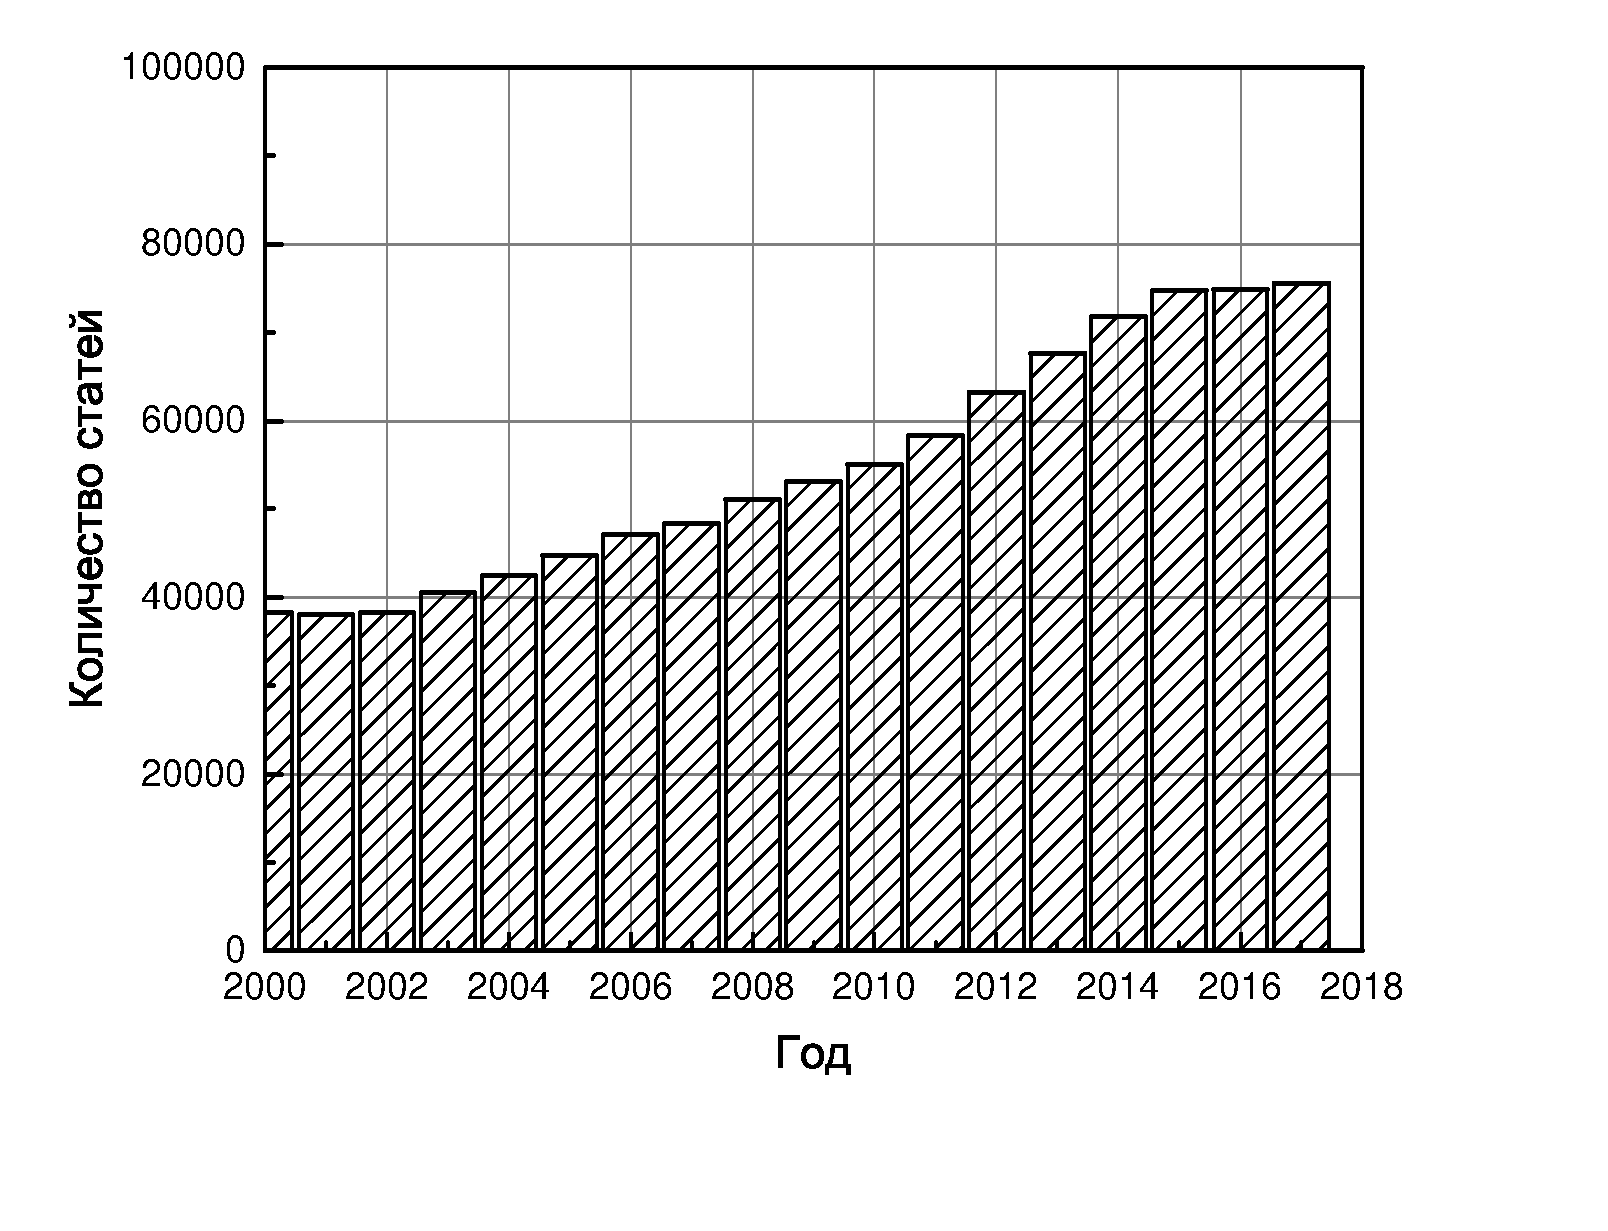
\includegraphics[width=1\linewidth]{1}}
	\caption{Зависимость количества научных статей на темы связанные с мозгом. Информация взята с ресурса  pubmed }
	\label{fig:1}
\end{figure}% это титульный лист
\newpage
\section{Структура работы}
Для реализации нашего проекта мы решили воспользоваться возможностями языка JavaScript. Наш проект состоит из двух важных моментов, над которыми мы в основном работали по отдельности. Интерактивная модель мозга, отображающая основные структуры мозга и обучающий тест, позволяющий пользователю оценить пробелу в знании. 

\textbf{ Главная страница }


\begin{figure}[H]
	\center{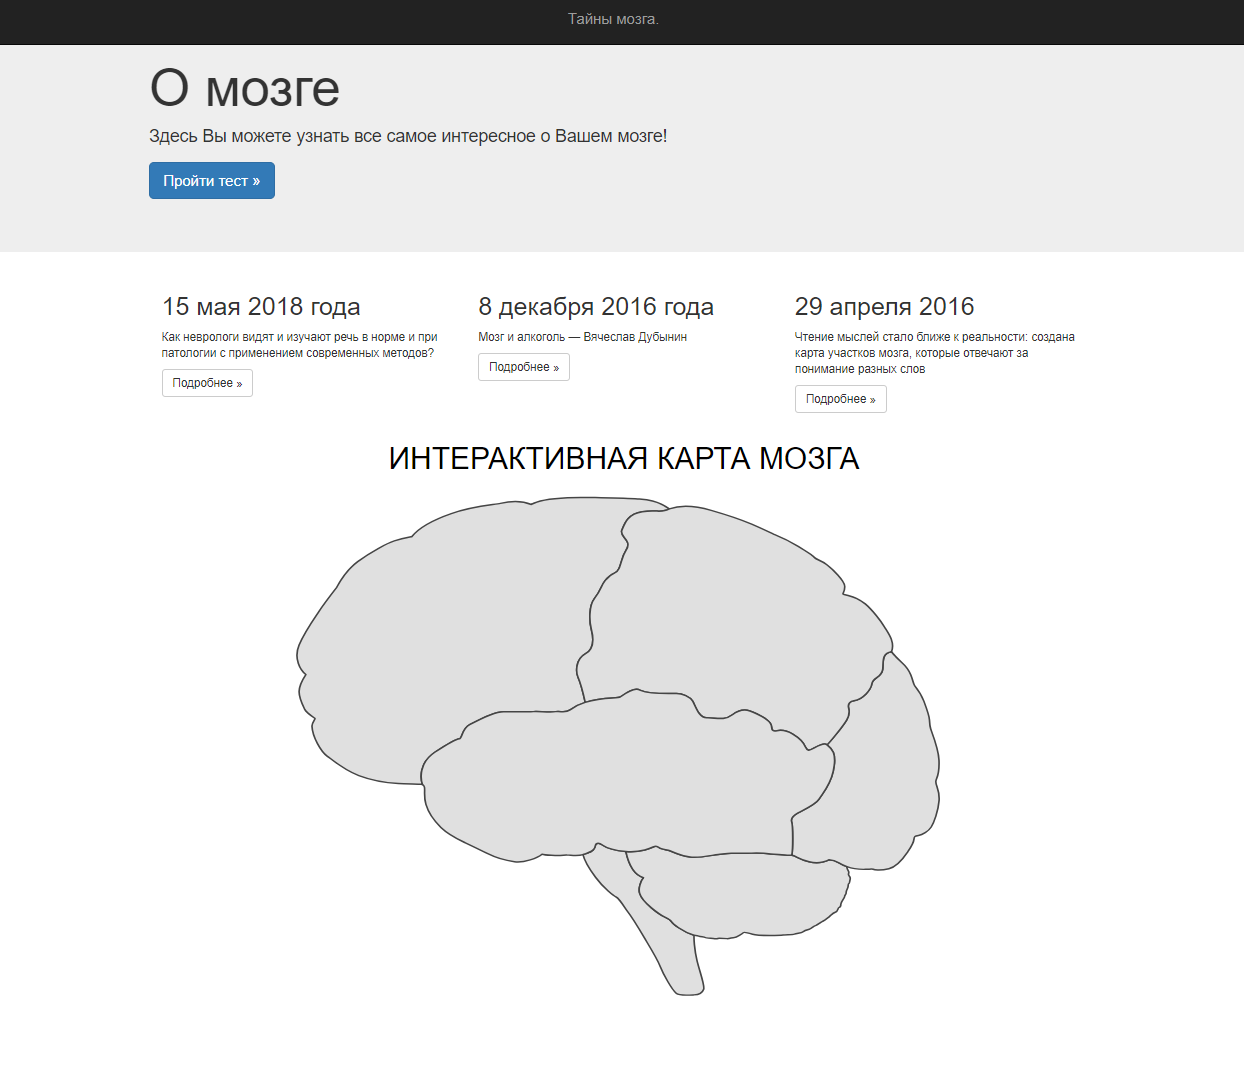
\includegraphics[width=1\linewidth]{8}}
	\caption{Главная страница ресурса}
	\label{ris:m}
\end{figure}


\subsection{Создание обучающего теста}
Созданием обучающего теста и сайта, на котором все расположено в основном занимался мой коллега, поэтому я не стану сильно распространяться, вы можете ознакомиться подробнее в его работе. 

Отмечу лишь несколько отличительных черт. Этот тест является не обычной проверкой знаний. Он носит образовательный характер из-за того что ответы даются пользователю сразу же после ответа и являются развернутыми ответами с примерами и доказательствами. За основу брались важные, на наш взгляд, заблуждения, связанные с работой мозга, о которых стоит знать правду.  




\subsection{Интерактивная карта мозга}
Изначальная задумка была, создать трехмерную интерактивную карту мозга, однако в последствии я пришел к выводу, что сделать это не представляется возможным в те сроки, что были отведены. Поэтому решили остановиться на 2д модели. Разумеется в качестве основы использовалось векторное изображение в формате SVG \footnote{Scalable Vector Graphics — масштабируемая векторная графика}, взятое из открытого источника. Векторное изображение позволяет масштабировать без потери качетсва, это то что нужно для наглядной демонстрации. Для построения карты мозга использовалась библиотека raphael, которая позволяет достаточно быстро и красиво отрисовать любую карту. Для обработки событий(интерактивности) использовалась библиотека jQuery. Карта выглядит следующим образом(рис.1). При наведении курсором мыши на область происходит её выделение. При нажатии появляется окошко, в котором представлена основная информация. Смотрите рис.2
\begin{figure}[h]
	\center{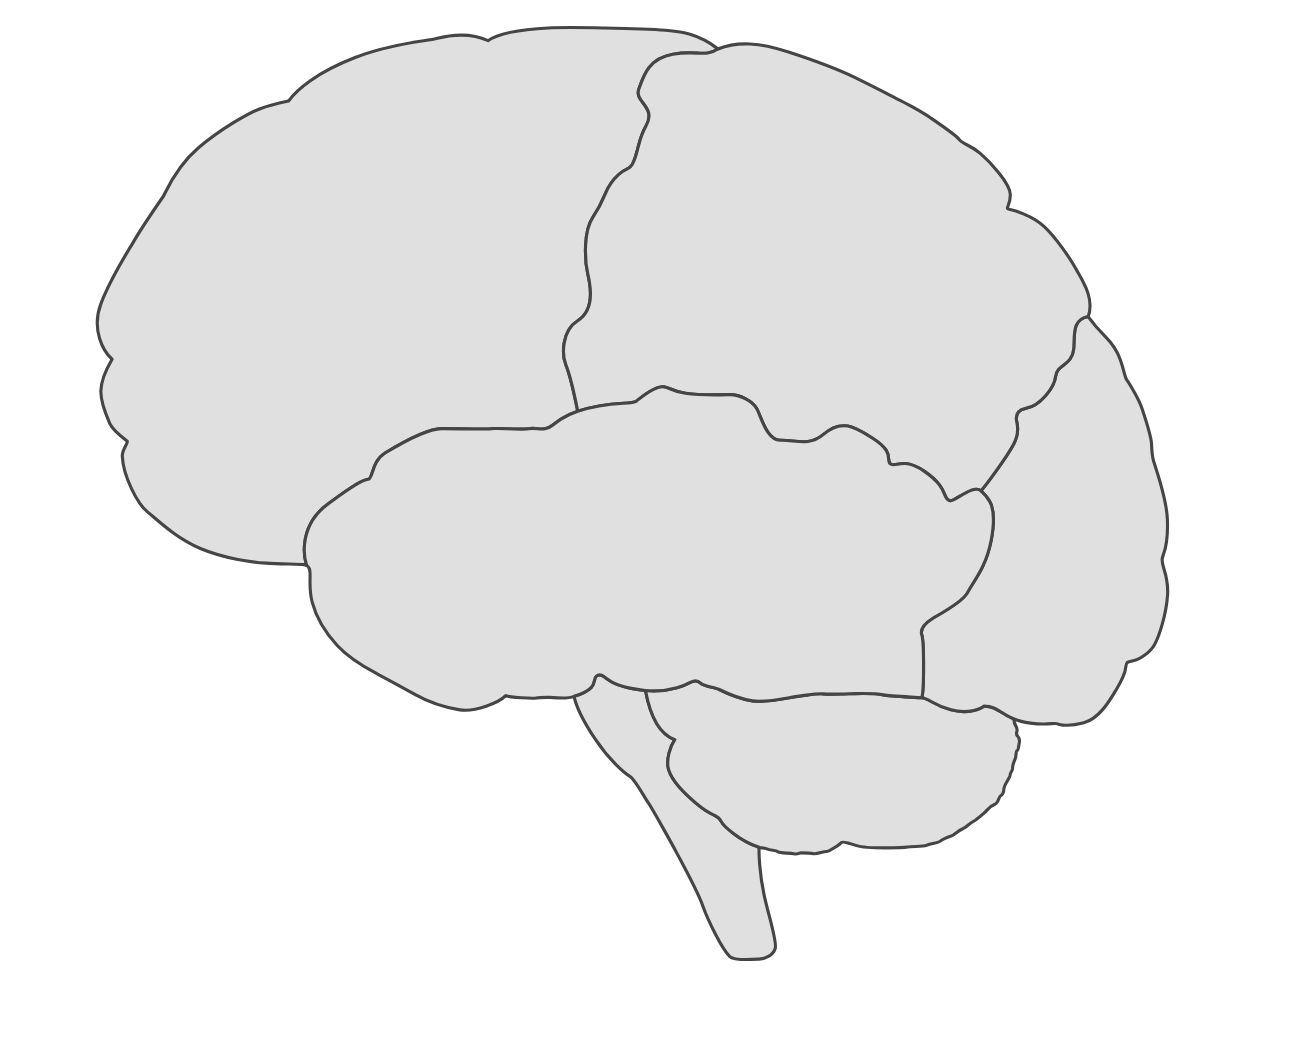
\includegraphics[width=0.8\linewidth]{4}}
	\caption{Карта мозга без взаимодействия}
	\label{fig:1}
\end{figure}
\begin{figure}[H]
	\center{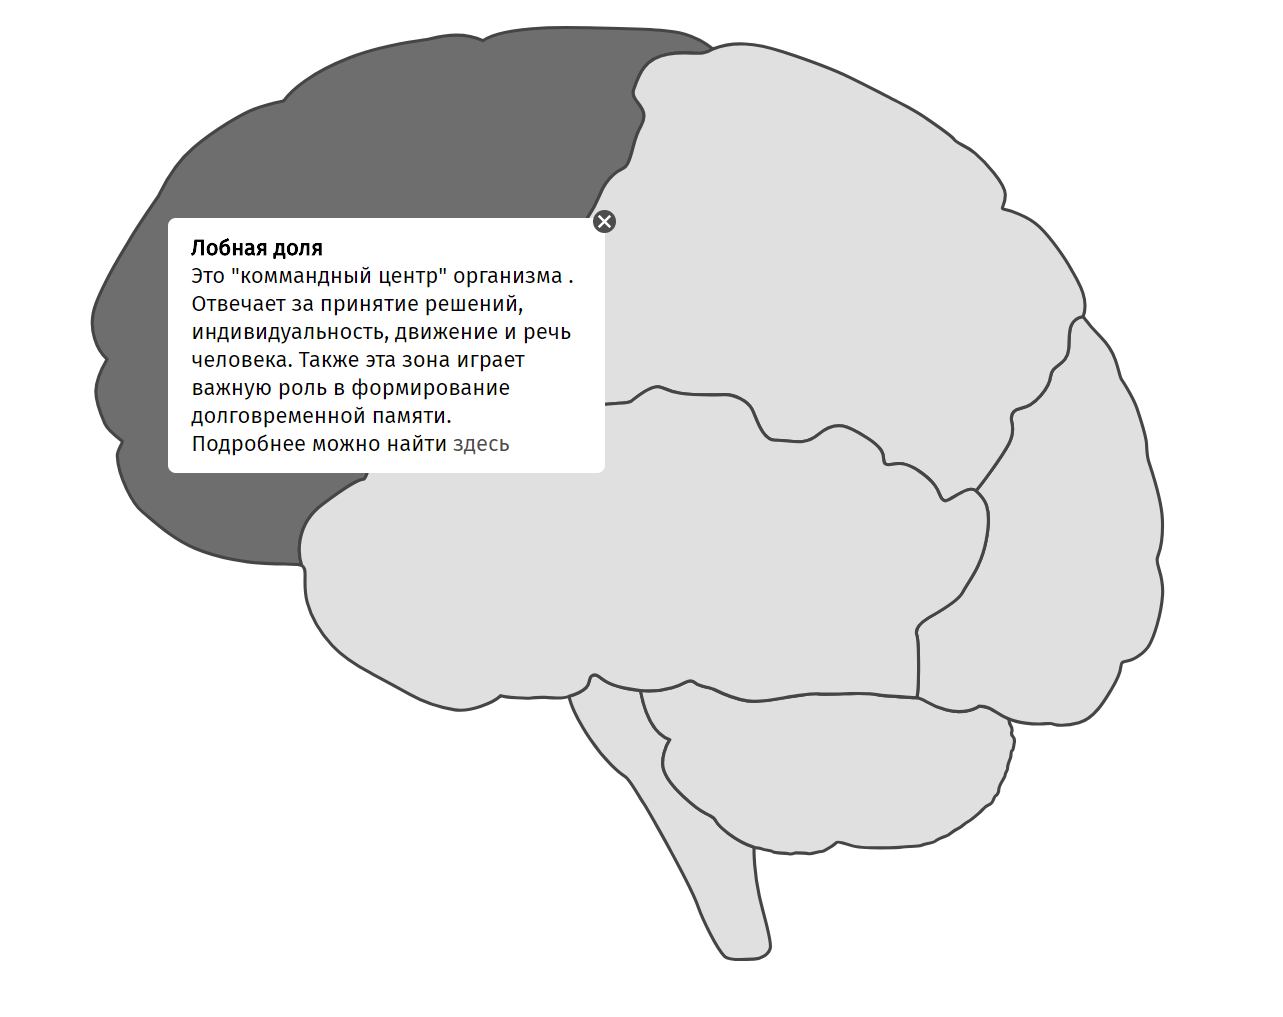
\includegraphics[width=0.8\linewidth]{2}}
	\caption{Карта мозга при нажатии курсора мыши}
	\label{fig:2}
\end{figure}

Теперь давайте поговорим более предметно, как происходит построение карты. Перво-наперво необходимо создать массив из различных зон, представленных в svg коде. Также каждому элементу массива присваивается информация об участке. Пример на рис. \ref{ris:mas}
\begin{figure}[h]
	\center{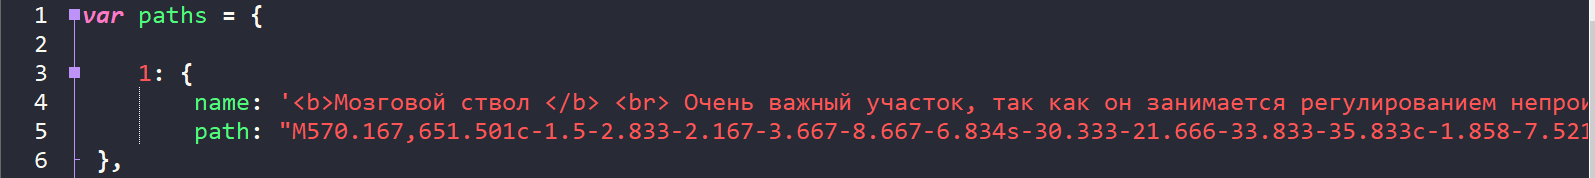
\includegraphics[width=1\linewidth]{5}}
	\caption{Элемент массива}
	\label{ris:mas}
\end{figure}

Далее происходит создание холста, определенного размера, на котором будет размещена наша карта, задаются специальные аттрибуты отрисовки(цвет заливки, цвет и ширина контура и размеры). 
После этого программа отрисовывает каждый контур с использованием заданных атрибутов, а также с помощью библиотеки jQuery взаимодействие. Вы можете видеть, что сначала прописывается действие при наведение курсора, а затем при нажатии. Также добавлена кнопка "закрыть", позволяющая скрыть окошко с информацией. Код представлен ниже, для того, чтобы сделать его более понятным написаны комментарии.
\begin{figure}[h]
	\center{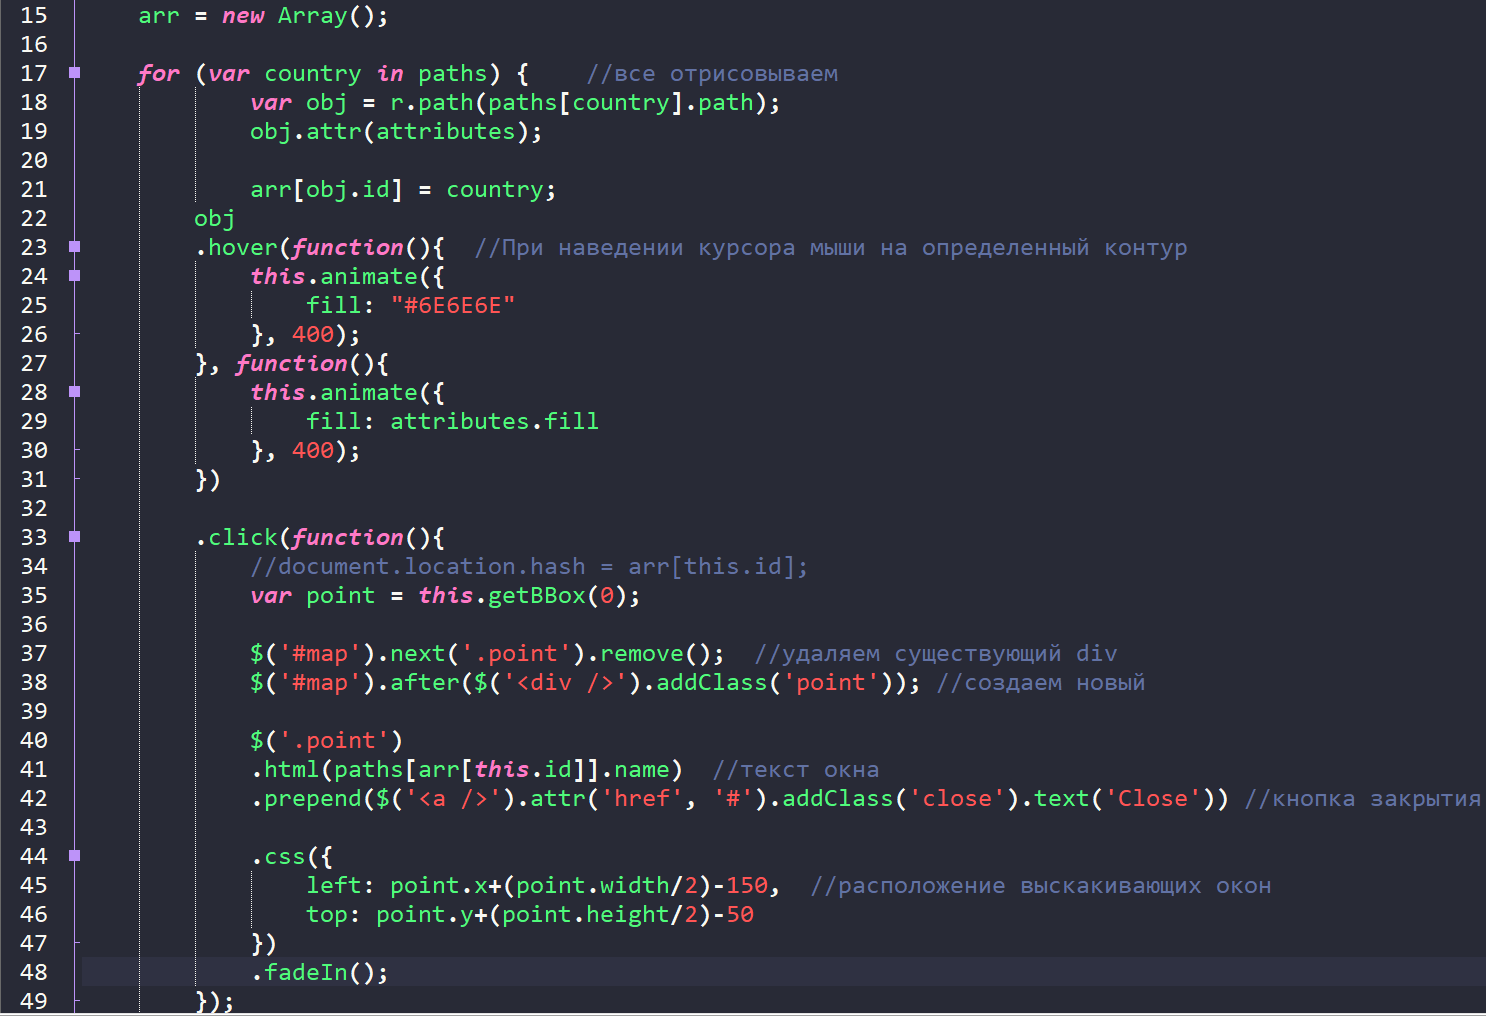
\includegraphics[width=1\linewidth]{6}}
	\caption{Отрисовка контуров, действия при наведении и при нажатии на контур}
	\label{ris:m}
\end{figure}

\begin{figure}[h]
	\center{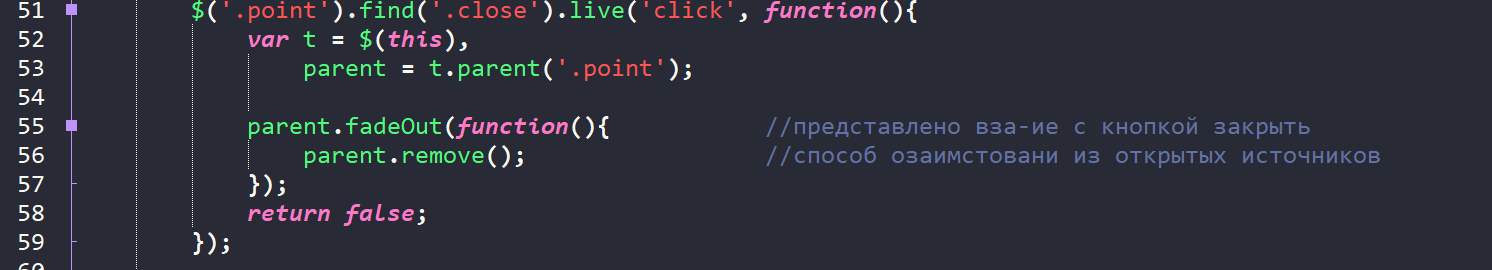
\includegraphics[width=1\linewidth]{7}}
	\caption{Работа кнопки закрыть}
	\label{ris:m}
\end{figure}



\section{Заключение}
В процессе выполнения работы, я познакомился со способами построения интерактивных карт, с возможностями библиотеки raphael и jQuery. Также я больше узнал о работе мозга, и о заблуждениях, о некоторых я даже не догадывался. Моим коллегой был составлен обучающий тест, а также сайт на котором всё располагается. Сервис получился довольно приятным в использовании. Мы очень надеемся на то, что проект принесет пользу для обычных пользователей и они смогут узнать что-то о самом сложном органе во вселенной. 






\end{document}
